% <text> Move to discussion
Previously, \textcite{baumgartnerFlavinbasedMetabolicCycles2018} did so by treating cells with the cell division cycle inhibitor rapamycin, while \textcite{papagiannakisAutonomousMetabolicOscillations2017} treated cells with the mating pheromone alpha factor to induce arrest in G1.

In contrast, I halt cell division cycles by changing nutrient conditions.
% </text>

% <text> Move to discussion
This observation is consistent with the knowledge on the cell division cycle, %[CITATION NEEDED]
and it draws comparison with the discussion about the change in lengths of phases in the metabolic cycle. %[ELABORATE MORE -- CONSULT INTRO.  I'm thinking of the Mellor/Slavov & Botstein stuff]
%THIS THEN WARRANTS DISCUSSION.
% </text>

% <text> Move to discussion
These discrepancies may be partly explained by the lack of information about cell-to-cell heterogeneity in the chemostat.
Chemostat studies commonly state that they induce metabolic cycles by imposing glucose starvation in the culture for some time.
In light of the glucose-starvation results in section~\ref{sec:biology-abrupt}, these metabolic cycles may be the combined effect of individual cells' response to starvation.
A lack of dissolved oxygen oscillations in zwf1$\Delta$ with a growth rate similar to wild-type \parencite{tuCyclicChangesMetabolic2007} may be explained by a loss of ability to reset the phase of the metabolic cycle or a variety of metabolic cycle lengths.
In addition, the M-shaped dissolved oxygen oscillations in tsa1$\Delta$ tsa2$\Delta$ may be explained by the combined effect of sub-populations that have different metabolic cycle periods.
These ideas are additionally supported by how my metabolic cycles are far shorter than the periods of chemostat-based metabolic cycles.
% </text>


% OLD HISTOGRAMS / KSTEST

\begin{figure}
  \centering
  \begin{subfigure}[htpb]{0.9\textwidth}
   \centering
   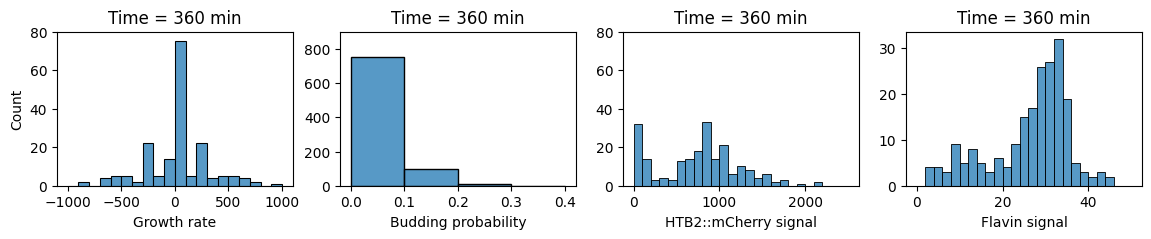
\includegraphics[width=\textwidth]{19972_distribs_0360}
   \caption{
     %foobar
     \SI{360}{\minute}
   }
   \label{fig:biology-starvation-distribs-0360}
  \end{subfigure}

  \begin{subfigure}[htpb]{0.9\textwidth}
   \centering
   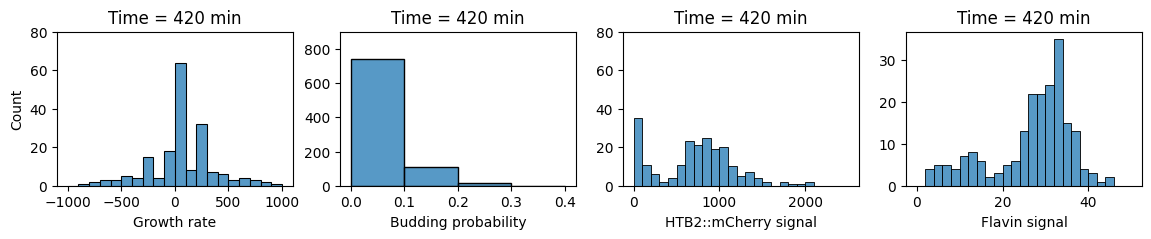
\includegraphics[width=\textwidth]{19972_distribs_0420}
   \caption{
     \SI{420}{\minute}
   }
   \label{fig:biology-starvation-distribs-0420}
  \end{subfigure}

  \begin{subfigure}[htpb]{0.9\textwidth}
   \centering
   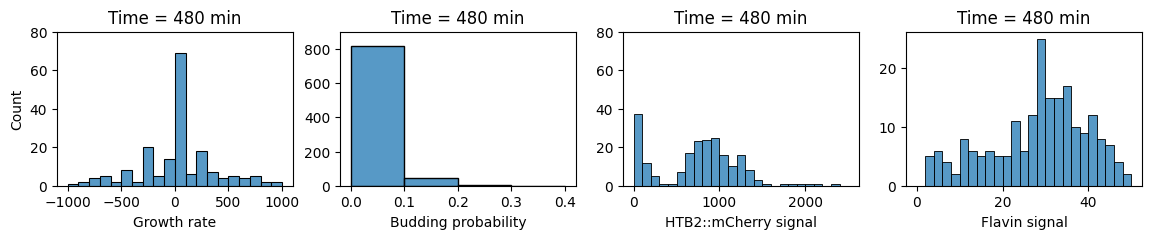
\includegraphics[width=\textwidth]{19972_distribs_0480}
   \caption{
     \SI{480}{\minute}
   }
   \label{fig:biology-starvation-distribs-0480}
  \end{subfigure}

  \begin{subfigure}[htpb]{0.9\textwidth}
   \centering
   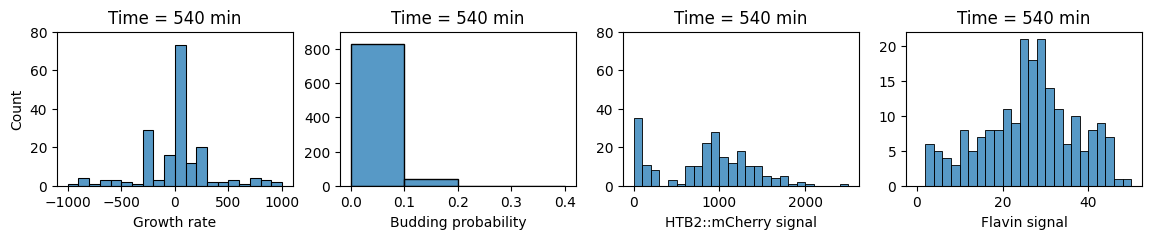
\includegraphics[width=\textwidth]{19972_distribs_0540}
   \caption{
     \SI{540}{\minute}
   }
   \label{fig:biology-starvation-distribs-0540}
  \end{subfigure}

  \begin{subfigure}[htpb]{0.9\textwidth}
   \centering
   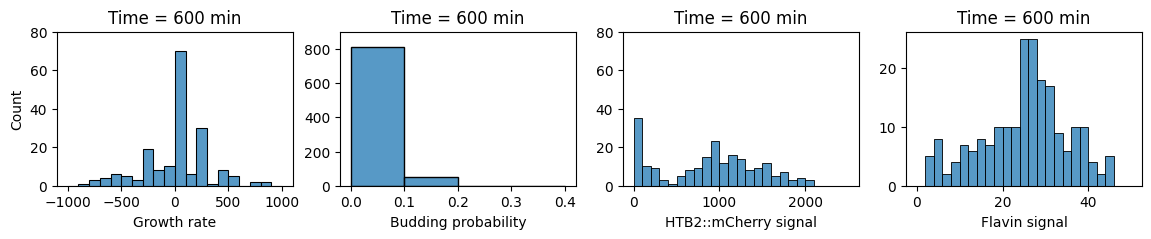
\includegraphics[width=\textwidth]{19972_distribs_0600}
   \caption{
     \SI{600}{\minute}
   }
   \label{fig:biology-starvation-distribs-0600}
  \end{subfigure}

  \begin{subfigure}[htpb]{0.9\textwidth}
   \centering
   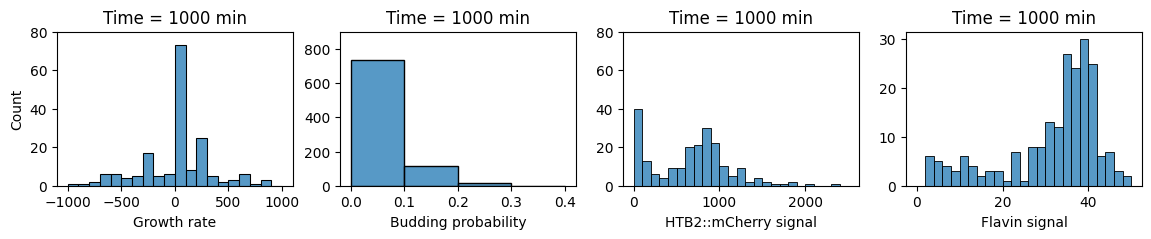
\includegraphics[width=\textwidth]{19972_distribs_1000}
   \caption{
     \SI{1000}{\minute}
   }
   \label{fig:biology-starvation-distribs-1000}
  \end{subfigure}

  \caption{
    Distribution of quantities at selected time points in the glucose-starvation experiment, starvation being \SIrange{420}{900}{\minute}.
    HTB2::mCherry and flavin signals were based on raw data extracted from the fluorescent images.
    Growth rate was calculated based on the rolling mean of the time point-to-time point change in cell volume estimated by \emph{aliby}, and the budding probability was calculated based on the rolling mean of the boolean vector that indicates the presence or absence of budding event over time.
  }
  \label{fig:biology-starvation-distribs}
\end{figure}


\begin{figure}
  \centering
  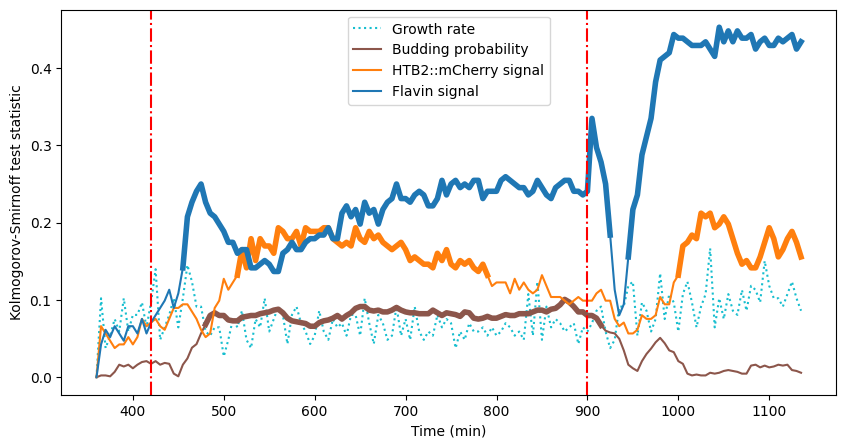
\includegraphics[width=\textwidth]{19972_ks_highlight}
  \caption{
    Glucose-starvation experiment.
    For each quantity, the Kolmogorov-Smirnov test statistics from two-tailed tests between the distribution at \SI{360}{\minute} and the distribution at each time point of interest is shown.
    The null hypothesis for each test is that the two samples are drawn from the same probability distribution, and thick lines indicate where the hypothesis is rejected ($p < 0.05$).
    Vertical lines (red) indicate changes in nutrient conditions.
  }
  \label{fig:biology-starvation-ks}
\end{figure}


% This sentence is difficult to understand.  Deal with it during the editing phase.
To extend information about the cell division cycle phase each cell is upon and during starvation across the population, I show the distribution of the raw HTB2::mCherry signals at time points of interest in the experiment (figure~\ref{fig:biology-starvation-distribs}).
The distributions of growth rates, budding probability, and raw flavin intensity are also shown.
To quantify how the distributions of these quantities change over time, I performed a two-tailed Kolmogorov-Smirnov test between a pre-starvation reference time each time point of interest over the course of the experiment (figure~\ref{fig:biology-starvation-ks}).

Consistent with figure~\ref{fig:biology-starvation-budprob}, the distribution of budding probability skews more towards zero during starvation, indicating sparse budding, and then budding resumes after starvation.
During starvation, initially the distribution of HTB2::mCherry signals remain the same, but after approximately \SI{2}{\hour}, it becomes more spread out.
This pattern suggests a delay in the effect of starvation on the progress of the cell division cycle as cell division cycles progress to their next available checkpoints.
Interestingly, the distribution of flavin signals skews to lower values during starvation, before recovering after starvation, and this suggests a more reduced cellular oxidation state during starvation.
% ...Needs more interpretation.  What does this suggest about the cell biology during starvation?  Is there a link to the literature?



\begin{figure}
  \centering
  \begin{subfigure}[htpb]{0.9\textwidth}
   \centering
   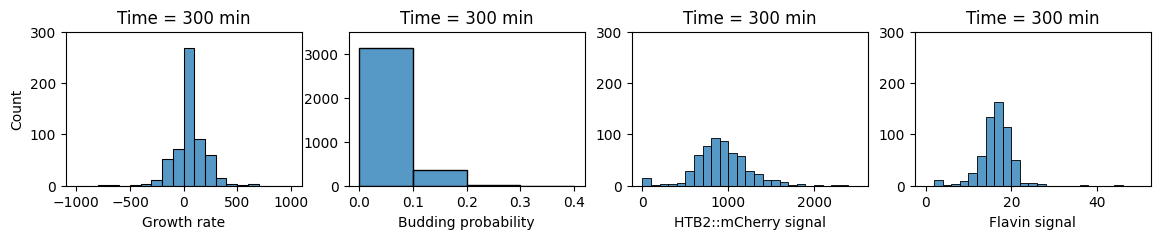
\includegraphics[width=\textwidth]{613_distribs_0300}
   \caption{
     \SI{300}{\minute}
   }
   \label{fig:biology-kdeficient-distribs-0300}
  \end{subfigure}

  \begin{subfigure}[htpb]{0.9\textwidth}
   \centering
   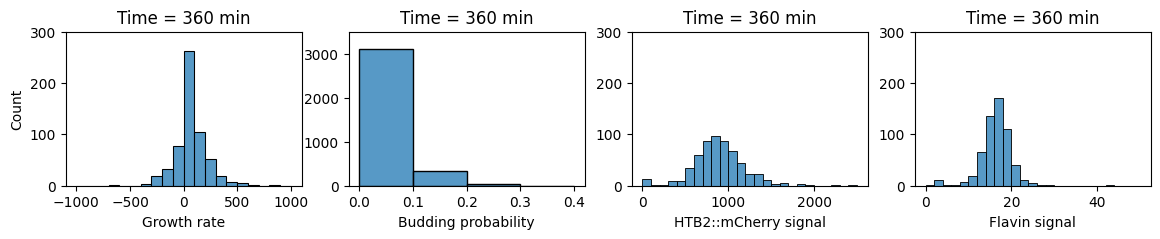
\includegraphics[width=\textwidth]{613_distribs_0360}
   \caption{
     \SI{360}{\minute}
   }
   \label{fig:biology-kdeficient-distribs-0360}
  \end{subfigure}

  \begin{subfigure}[htpb]{0.9\textwidth}
   \centering
   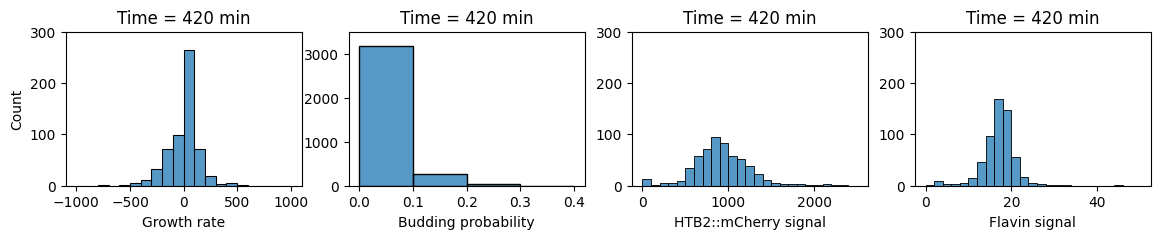
\includegraphics[width=\textwidth]{613_distribs_0420}
   \caption{
     \SI{420}{\minute}
   }
   \label{fig:biology-kdeficient-distribs-0420}
  \end{subfigure}

  \begin{subfigure}[htpb]{0.9\textwidth}
   \centering
   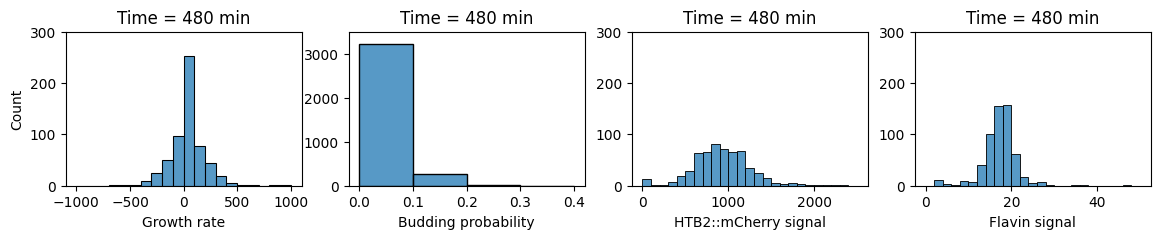
\includegraphics[width=\textwidth]{613_distribs_0480}
   \caption{
     \SI{480}{\minute}
   }
   \label{fig:biology-kdeficient-distribs-0480}
  \end{subfigure}

  \begin{subfigure}[htpb]{0.9\textwidth}
   \centering
   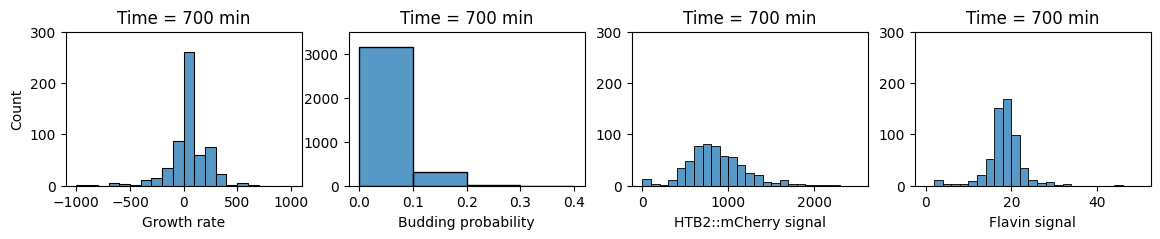
\includegraphics[width=\textwidth]{613_distribs_0700}
   \caption{
     \SI{700}{\minute}
   }
   \label{fig:biology-kdeficient-distribs-0700}
  \end{subfigure}

  \begin{subfigure}[htpb]{0.9\textwidth}
   \centering
   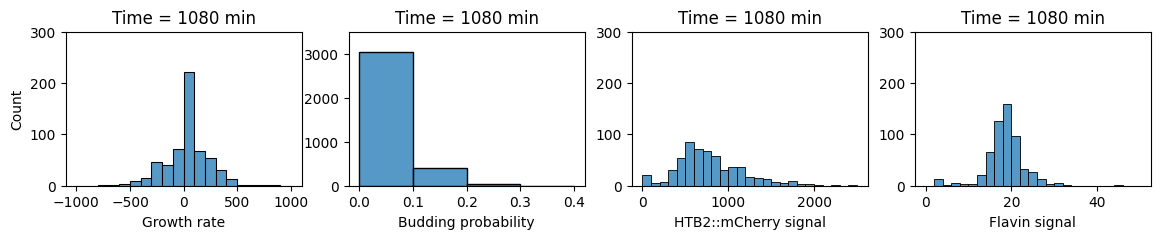
\includegraphics[width=\textwidth]{613_distribs_1080}
   \caption{
     \SI{1080}{\minute}
   }
   \label{fig:biology-kdeficient-distribs-1080}
  \end{subfigure}

  \caption{
    Distribution of quantities at selected time points in the potassium-deficiency experiment, potassium-deficiency being \SIrange{360}{960}{\minute}.
    HTB2::mCherry and flavin signals were based on raw data extracted from the fluorescent images.
    Growth rate was calculated based on the rolling mean of the time point-to-time point change in cell volume estimated by \emph{aliby}, and the budding probability was calculated based on the rolling mean of the boolean vector that indicates the presence or absence of budding event over time.
  }
  \label{fig:biology-kdeficient-distribs}
\end{figure}


\begin{figure}
  \centering
  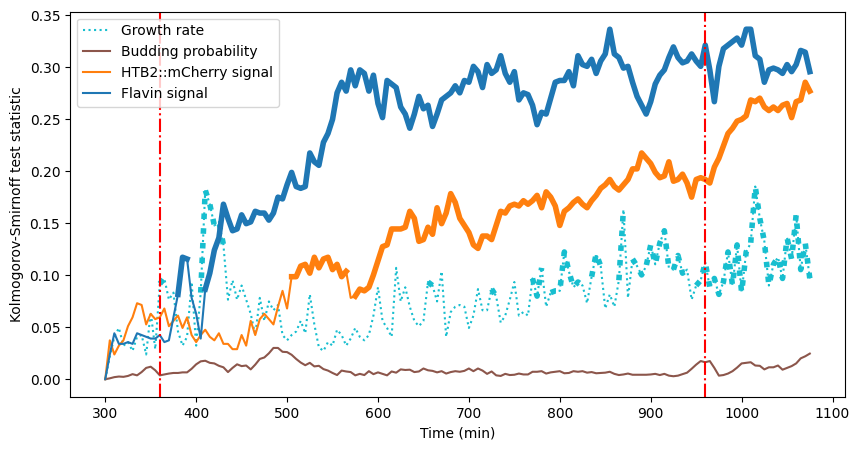
\includegraphics[width=\textwidth]{613_ks_highlight}
  \caption{
    Potassium-deficiency experiment.
    For each quantity, the Kolmogorov-Smirnov test statistics from two-tailed tests between the distribution at \SI{300}{\minute} and the distribution at each time point of interest is shown.
    The null hypothesis for each test is that the two samples are drawn from the same probability distribution, and thick lines indicate where the hypothesis is rejected ($p < 0.05$).
    Vertical lines (red) indicate changes in nutrient conditions.
  }
  \label{fig:biology-kdeficient-ks}
\end{figure}

% Conclusions are a bit iffy.  I probably need to think of new statistical tests.
As for the glucose-starvation experiment, I then investigated how the distribution of growth rates, budding probability, raw HTB2::mCherry intensity, and raw flavin intensity changes over the course of the experiment (figures~\ref{fig:biology-kdeficient-distribs},~\ref{fig:biology-kdeficient-ks}), using the \SI{300}{\minute} time point as the pre-potassium-deficiency reference point.
In contrast to the glucose-starvation experiment, the distribution of budding probability never showed a significant change from the pre-deficiency reference point throughout the experiment.
Additionally, the growth rates changed distribution profile when the growth rates dropped in the initial response to potassium depletion, and again later in the potassium-deficient condition.
Interestingly, the distribution of HTB2::mCherry intensities become more spread towards the end of the experiment, while the mean value of flavin intensity did not change as drastically at it did for the glucose-starvation experiment.



% DELETION STRAINS


They interpret that entry into the pentose phosphate pathway, and thus production of NADPH, is required for the metabolic cycle.
\textit{ZWF1} codes for glucose-6-phosphate dehydrogenase, a key metabolic enzyme in the pentose phosphate pathway that plays a role in production of NADPH, which is a key player in YMC.
% ELABORATE MORE -- TAKE FROM ZWF1 ORG NOTE
Though, it is important to note that ALD6 and IDP2 can compensate this NADPH production \parencite{minardSourcesNADPHYeast2005}.

The double deletion affects a pair of paralogous genes that are involved in redox metabolism (key player of metabolic cycle), linked to circadian rhythm (another biological rhythm), therefore it was targeted as a potentially important gene for the metabolic cycle.


% DISCUSSION

%This is consistent with \textcite{oneillEukaryoticCellBiology2020} and (add other citations here).
Cross-correlation between flavin and mCherry signals further confirm the sequence of events while the two biological oscillations (metabolic cycle and cell division cycle) progress.
This relationship is particularly obvious in pyruvate.
Specifically, when the new bud forms, the mother cell's flavin fluorescence peaks.
Subsequently, the cell synthesises new histones in S phase, then the cell enters anaphase --- characterised by the sharp drop in the mCherry signal --- as the flavin fluorescence is at its trough.

This chapter additionally shows that cells individually generate metabolic cycles and individually adapt them in response to nutrient changes.
The literature disputes whether metabolic oscillations arise from interactions between cells or whether cells individually generate oscillations.
In my observations, even though the cells are physically separated in traps and nutrient media flows through them, single-cell flavin oscillations can synchronise and reset phase in certain conditions.
Diffusible metabolites cannot be responsible.
I thus conclude that each cell --- on its own --- can reset its metabolic cycle in response to nutrient changes.
This conclusion does not mean that cells \emph{cannot} communicate with each other, but communication is \emph{not required}.

Observations of the two oscillators during starvation piques curiosity about their mechanistic basis in such conditions.
% TODO: Come up with new analysis to prove/disprove this.  Or link this with existing results.  It's still quite unclear to me.
For the cell division cycle, the most likely explanation is if starvation occurs before START, cell remain in pause; if starvation occurs after START, cells go into pause.
In contrast, the biochemical mechanism that the cell uses to reset the phase of its metabolic cycle, is unclear, and it owes to the poor characterisation of the biochemistry of the metabolic cycle in general.

This chapter also attempts to reconcile chemostat and single-cell studies.
In chemostats, glucose is limiting \parencite{jonesCyberneticModelGrowth1999}.
Synchrony of metabolic cycles between cells in respiring conditions may explain observations in chemostat as cells are near glucose starvation in these conditions.

Single-cell metabolic cycles in zwf1$\Delta$ are inconsistent, and this may explain the absence of dissolved-oxygen oscillations in the chemostat.
zwf1$\Delta$ affects many metabolic processes; most notably, it removes a major pathway of NAD(P)H generation from reduction of NAD(P)\textsuperscript{+}.
The most abundant flavoproteins involve NAD(P)H redox, so it is reasonable to believe that flavin oscillations are affected.
Perhaps zwf1$\Delta$ impairs the metabolic cycle in some way.
A similar logic likely applies to tsa1$\Delta$ tsa2$\Delta$ --- perhaps the interaction between a more variable length of metabolic oscillations interacts with population synchrony, or lack thereof, in the chemostat.
Furthermore, the tsa1$\Delta$ tsa2$\Delta$ double deletion affects the peroxiredoxin-thioredoxin system, therefore affecting redox balance, likely in an extensive way.

The fact that metabolic oscillations are present when the medium is potassium-free can be seen as more evidence that there is no straight one-to-one correspondence between dissolved-oxygen metabolic oscillations in the chemostat and single-cell flavin oscillations from single cells.
Therefore, the difference between single-cell and chemostat traces warrant a model to explain the differences, likely involving subpopulations.
My observations thus also highlight a weakness of chemostat experiments.
